The dielectric SiN membranes have extraordinary optical properties such as low absorption \cite{Wilson2011}, but it lacks a bit in reflectivity. The dielectric membrane with thickness $d$ has the electric field reflectivity coefficient $r_m$ and transmission coefficient $t_m$ \cite{jayich2008, Wilson2011}

\begin{align}
  \label{eq:mem_opt_prop}
  r_m & = \frac{(n^2 -1)\sin(knd_m)}{2in\cos(knd) + (n^2 +1)\sin(knd)} \\
  t_m & = \frac{2n}{2in\cos(knd) + (n^2 +1)\sin(knd)},
\end{align}
\noindent
where $n$ is the index of refraction of the dielectrics and $k$ is the wavenumber of the light incident on the membrane. In figure \ref{fig:mem_prop} we show the reflectivity coefficient $r_m$ as a function of refractive index $n$, which is also equivalent to increasing the thickness $d$. We also plot $r_m$ for a realistic index of refraction $n = 2$ \cite{Wilson2011} and vary the wavelength in figure \ref{fig:mem_prop}.

\begin{figure}[H]
\centering
    \begin{subfigure}[b]{0.49\textwidth}
    \centering
    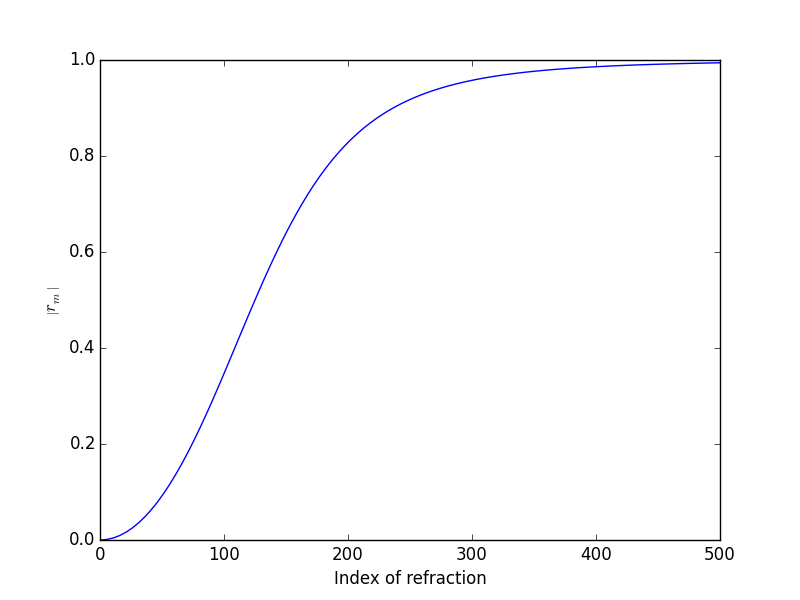
\includegraphics[width=\textwidth]{mem_ref_vs_index_of_refrac.png}
    \caption{}
    \label{fig:mem_ref_refrac}
    \end{subfigure}
    \hfil
    \begin{subfigure}[b]{0.49\textwidth}
    \centering
    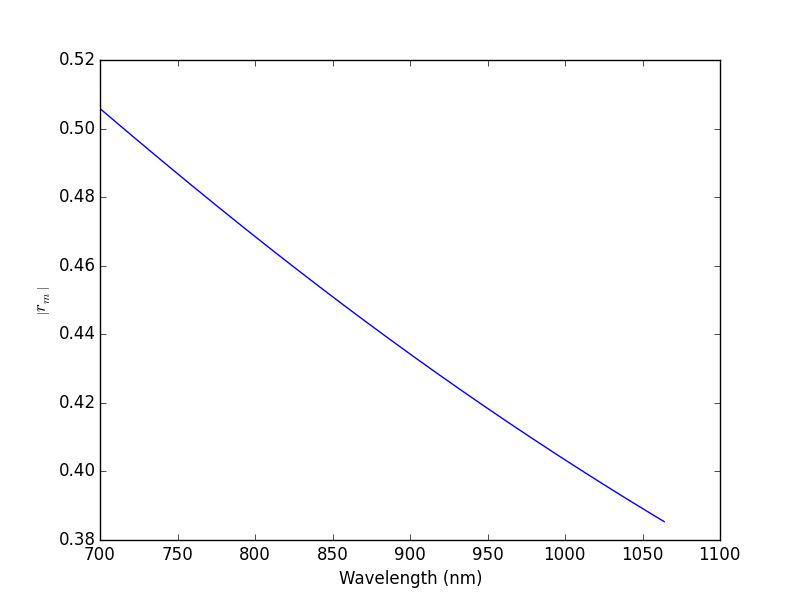
\includegraphics[width=\textwidth]{mem_ref_vs_wavelength.png}
    \caption{}
    \label{fig:mem_ref_wavelength}
    \end{subfigure}
\caption{(a) Membrane reflectivity coefficient $r_m$ as a function of index of refraction $n$. (b) Reflectivity coefficient $r_m$ as we change the wavelength of the light for fixed index of refraction $n = 2$.}
\label{fig:mem_prop}
\end{figure}